\section{Experiments for 2048}

\subsection{Design of N-tuple Networks and Vertical Split Encoding}

% 6, 7, 8, 9 タプルをデザインした.デザインにあたっては,「妥当そうに見える形を人手で設計し,それらを平行移動する」ヒューリスティクスを用いた.
% 6タプル NT6 では,4つの形を選定し,それらを平行移動してできる9つの組合せとした.
% 7タプル NT7 では,4つの形を選定し,それらを平行移動してできる8つの組合せとした.
% 8タプル NT8 では,3つの形を選定し,それらを平行移動してできる5つの組合せとした.
% 9タプル NT9 では,4つの形を選定し,それらを平行移動してできる7つの組合せとした.
% baseline として,先行研究で用いられていた 8x6-tuples からなるネットワーク NT6-M を用いる.

Table~\ref{fig:NTupleVSE} summarizes the design of N-tuple networks and Vertical Split Encoding
used in our experiments for 2048.

By adopting the heuristics of ``manually creating reasonable shapes and generating their translations''~\cite{Jask18}, we designed new sets of N-tuple networks for 6-, 7-, 8-, and 9-tuple cases.
\begin{itemize}
\item \textsf{NT6}: We designed four shapes of 6-tuples and obtained nine tuples by their translations.
\item \textsf{NT7}: We designed four shapes of 7-tuples and obtained eight tuples by their translations.
\item \textsf{NT8}: We designed three shapes of 8-tuples and obtained five tuples by their translations.
\item \textsf{NT9}: We designed four shapes of 9-tuples and obtained seven tuples by their translations.
\end{itemize}
As a baseline, we used \textsf{NT6-M}, a network consisting of 8$\times$6-tuples, which was first selected through intensive experiments by Matsuzaki~\cite{Mats16} and employed in the state-of-the-art player by Guei et al.~\cite{GuCW22}.

% それぞれの N-Tuple について,各パラメータを 64 bits とし,3倍のメモリを必要とする TC 学習と,2倍のメモリを必要とする multi-staging を用いても64 GBメモリに収まることを要件として,VSE の value ranges を設計した.
% 6タプルからなる NT6 と NT6M の場合は VSE なしで十分メモリに収まる.
% 7タプルからなる NT7 の場合には,少なくとも 2 つに分ける必要があり,2つのvalue ranges の大きさが 11 + 10 となるように分けた.
% 8タプルからなる NT8 の場合には,少なくとも 3 つに分ける必要があり,3つのvalue ranges の大きさが 9 + 9 + 6 となるように分けた.
% 9タプルからなる NT9 の場合には,少なくとも 4 つに分ける必要があり,4つのvalue ranges の大きさが 7 + 7 + 7 + 6 となるように分けた.
For each set of N-tuples, we designed the VSE value ranges under the following assumptions: each element in lookup tables has 64 bits; we use temporal coherence learning~\cite{Jask18} that requires three times as much memory with three lookup tables; and we use multi-staging technique with two stages~\cite{GuCW22} that requires two times as much memory; the whole training program should fit within 64 GB of memory.
Our final design of VSEs was as follows.
\begin{itemize}
\item For \textsf{NT6} and \textsf{NT6-M}, the parameters sufficiently fit within the memory without VSE, and so we do not apply VSE.
\item For \textsf{NT7}, at least two splits are needed, and thus we use 2-VSE with two value ranges of sizes 11 and 10.
\item For \textsf{NT8}, at least three splits are needed, and thus we use 3-VSE with three value ranges of sizes 9, 9, and 6.
\item For \textsf{NT9}, at least four splits are needed, and thus we use 4-VSE with four value ranges of sizes 7, 7, 7, and 6.
\end{itemize}

% VSE の value ranges の取り方はもう少し自由度がある.それらを網羅的に試すのは今後の課題である.
Note that there exist a few more flexibility in the choice of value ranges of VSE.
Exhaustively exploring those possibilities remains as future work.

\subsection{Training and Evaluation with 1-ply Lookahead Play}

% 上のように定義した N-tuple networks に対し,強化学習によってパラメータを調整した.
% 学習には,Optimistic initialization ありの Temporal Coherence 学習を用いた.
% Temporal coherence 学習(TC 学習):学習率を自動的に調整する機能を備えた TD 学習であり、Jaśkowski によって初めて 2048 に導入された手法である。本研究における N タプルネットワークの学習では、効率的かつ安定的な収束のために TC 学習を採用した。
% Optimistic initialization(OI):学習初期段階での探索を広く行うために、重みをゼロではなく大きな値で初期化する手法である。本研究では、すべての afterstate の初期値が 320,000 となるように重みを初期化した。
% OI 以外には,Exploration は入れていない.局所最適にならないよう,TC 学習で学習率を決定するパラメータを初期化する.$50 x 10^9$ step ごと.
% また,先行研究にならって,ゲームの進行に応じて重みを参照するテーブルを切り替える multi-staging 手法を用いる。本研究では 2 ステージから構成し、タイル 32768 が生成される前後でネットワークを切り替える.

For the N-tuple networks with VSE defined above, we conducted reinforcement learning to tune their parameters.
In this study, we employed Temporal Coherence learning with Optimistic Initialization and Restart Strategy.
\begin{description}
 \item[Temporal Coherence learning~\normalfont{\cite{Jask18}}] Temporal Coherence learning (TC learning) is a variant of TD learning that enables automatic adjustment of the learning rate, which was first introduced to 2048 by Ja\'skowski.  To keep the effect of the following Optimistic Initialization, we decayed the learning rate from 0.5.
 \item[Optimistic Initialization~\normalfont{\cite{GuCW22}}] Optimistic Initialization (OI) is a method of encouraging exploration in the training by initializing the parameters with large values.  In this study, we use the same initial values as Guei et al.~\cite{GuCW22}: we initialize the parameters such that all afterstates have values of 320\,000.
 \item[Restart Strategy~\normalfont{\cite{Mats17}}] The games of 2048 are easy at the beginning but hard when the board is filled with large-number tiles.  To address this issue, we applied the restart strategy with constant number 10 of restarts.
 \item[Multi-staging~\normalfont{\cite{YWHC16}}] Following prior work~\cite{GuCW22}, we also employed the multi-staging method, in which the lookup tables are switched depending on game progression. In this study, we split the game into two stages, switching the lookup tables before and after the generation of a 32\,768 tile.
\end{description}
We introduced no additional exploration in the training apart from OI.
To avoid convergence to local optima, we reset the parameters controlling the learning rate in TC learning every $50 \times 10^9$ steps.

% 本研究における学習は,6,7,8,9のそれぞれのタプルと既存研究で用いたタプルの5種類についてそれぞれ$200 x 10^11$ step分学習を行う.$1x10^9$ ごとにパラメータを出力し,1-ply lookahead (Greedy) プレイ 10000 ゲームの平均得点をモニターした.
% なお,random 要素の対応として,5つの異なるseedを用いて学習を行い,そられの平均と標準偏差を求めた.
In this study, for each of five types of N-tuple networks above, we conducted the training for $200 \times 10^{9}$ steps.  During the training, we output the snapshot of the parameters every $1 \times 10^9$ steps and evaluate their performance in terms of the average score of 10\,000 games with 1-ply lookahead (greedy) play.
To mitigate the randomness, we conducted the training with five different random seeds, and report their means and standard deviations.

% 図 \ref{fig:exp2} にtraining curve を示す.
% $200x10^9$ steps 学習した最終結果の平均得点を見ると,NT8 > NT7 > NT9 > NT6 $\approx$ NT6-M となっている.
% NT8 の標準偏差がとても大きくなっているのは,2つのseedが平均得点約 40万,残りの3つが約 32万 と大きく異なったためである.これら悪い場合をとっていても,NT6 と NT6-M よりも高得点である.
% NT7 と NT9 については,NT6 と NT6-M からの差が標準偏差よりも十分に大きい.したがって,N-Tuple のサイズを大きくすることで有意に性能向上したと言える.
% 学習の経過についてより詳しく見ると,NT7 だけが他のネットワークと学習曲線の形が異なっている.
% NT7 の学習が他よりも遅かった理由について,タプルの形によるものか,2-VSE によるものか,現時点では分かっていない.
% また,もう一つ面白い点として,TC学習による学習率をリセットしたとき,タプルサイズが大きいもののほうがスコアの下がり方が小さい.
Figure~\ref{fig:exp2} shows the training curves.
The final average scores after the training with $200 \times 10^9$ steps were ranked as \textsf{NT8} $>$ \textsf{NT7} $>$ \textsf{NT9} $>$ \textsf{NT6} $\approx$ \textsf{NT6-M}.
The standard deviation for \textsf{NT8} was very large because training with two seeds succeeded achieving average scores of around 400\,000, while training with the other three saturated at around 320\,000.
Even considering these poor cases, \textsf{NT8} still outperformed \textsf{NT6} and \textsf{NT6-M}.
For \textsf{NT7} and \textsf{NT9}, the differences from \textsf{NT6} and \textsf{NT6-M} were sufficiently larger than their standard deviations.
These results indicated that increasing the N-tuple size with the help of VSE significantly improved performance.

A closer look at the training progress reveals that when the learning rates were reset in TC learning, networks with larger tuples showed smaller drops in score. This means that the training could be more stable with larger tuples but at the same time they tend to converge local optima.
Another interesting observation was that \textsf{NT7} was the only networks with a learning curve with a different shape.  Possible reasons for that slower learning would come from its tuple design or the use of 2-VSE, but we have no clear evidences so far.

\begin{figure}[ht]
 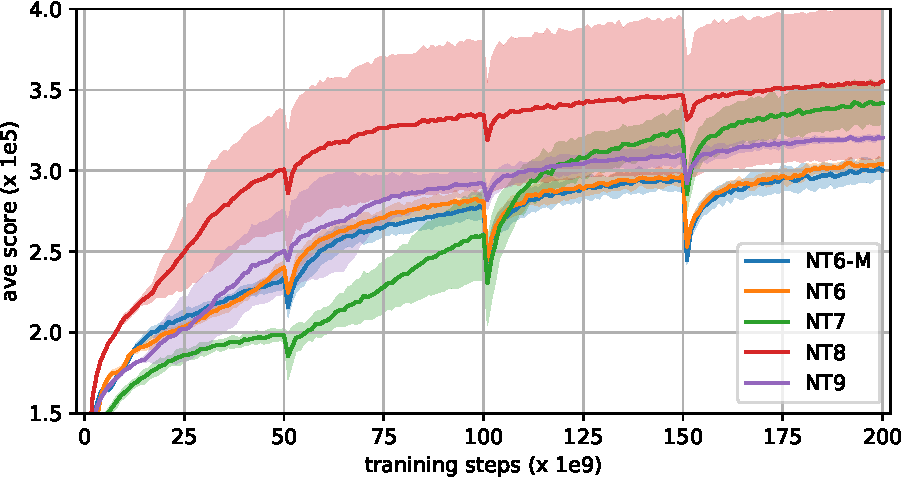
\includegraphics[width=.98\linewidth]{figures/plot-exp2.pdf}
 \caption{Training curve evaluated with 10000 games of 1-ply lookahead (greedy) play. The shaded areas show the standard deviations over five training runs.}
 \label{fig:exp2}
\end{figure}

\subsection{Evaluation with Expectimax Search}
% 最終的に得られたN-tuple network を用いて,Expectimax 探索 (3-ply, 5-ply) と組合せた評価も行った.
% 結果を \ref{table:exp3} に示す.
% 平均得点だけを見ると,3-ply や 5-ply のExpectimax探索を組み合わせたときに,NT6 や NT6-M を超える平均得点
% だったのは NT7 だけである.NT9 では,探索を組み合わせてもほとんど性能向上がない.
% とくに,32768 のタイルの生成率がすべて 0.0 \% となってしまっている.
% これは,lookup table のパラメータ数が多すぎるため局所最適な解へと学習してしまったことが原因と思われる.
% NT8 についても,学習がうまくいって1-ply で平均40万点であるものはExpectimax 探索で性能向上しているものの,
% 学習が停滞したものについては NT9 と同様に32768タイルの到達に失敗してしまっている.
% これにより,平均得点および32768タイルの到達率それぞれ標準偏差が非常に大きい結果となっている.
We also evaluated the final N-tuple networks in combination with Expectimax search (3-ply and 5-ply).
The results are shown in Table~\ref{table:exp3}.

\begin{table}[ht]
 \caption{Average scores and the ratios of reaching a 32\,768-tile for the networks trained over $200\times 10^9$ steps, evaluated with 1-ply lookahead (greedy) play and with Exxpectimax search with 3-ply and 5-ply lookahead. For each case, mean and standard derivation over five training runs (after $\pm$ sign) are given.}
 \label{table:exp3}
 \centering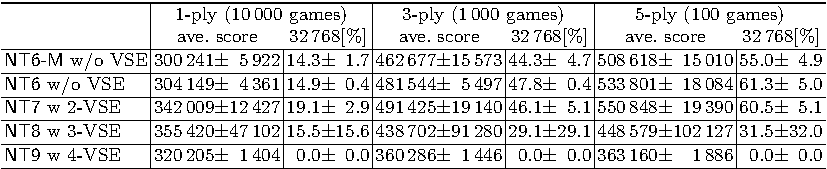
\includegraphics[width=.99\linewidth]{figures/table-exp3.pdf}
\end{table}

Looking only at the average scores when combined with 3-ply or 5-ply Expectimax search, \textsf{NT7} was the only network that outperformed \textsf{NT6} and \textsf{NT6-M}.
For \textsf{NT9}, the addition of search provided almost no improvement in performance. In fact, the generation rate of the 32\,768 tile was 0.0\% in all cases of \textsf{NT9}. This is likely due to overfitting: the lookup table contained too many parameters, causing the network to converge to local optima that fail to reach a 32\,768 tile.
For \textsf{NT8}, if training was successful (achieving around 400\,000 points in 1-ply play), the combination of Expectimax search further improved performance. However, when training saturated, \textsf{NT8} exhibited behavior similar to \textsf{NT9}, failing to reach a 32\,768 tile. As a result, both the average score and the 32\,768-tile reaching rate showed very large standard deviations.

\subsection{Evaluation of Best N-tuple Networks}

% 特に,NT8 で学習がうまくいったものとうまくいかなかったものがあったので,局所最適に陥いってしまったNT9を除くそれぞれのN-Tupleの大きさについて,5つの学習のうちもっともうまくいったネットワークを用いての評価を行った.
% 1つのネットワークに対して,5つの異なるシードでテストプレイ (1-ply, 3-ply, 5-ply) を行った結果を表 \ref{table:exp4} に示す.

% best ネットワークを用いた結果では,NT8 > NT7 > NT6 $\approx$ NT6-M となった.
% 5-ply の探索を組み合わせた場合についても,NT8 と NT6-M との差は7万点と標準偏差と比べて十分に大きな差が得られいる.
% したがって,VSE を組合せることでタプルサイズを大きくすることは,非常に有効だと結論付ける.

Since \textsf{NT8}, in particular, produced both successful and unsuccessful training outcomes, we conducted an additional evaluation using the best-performing networks for each N-tuple size, excluding \textsf{NT9}.
For each selected network, we ran test plays (10\,000 games with 1-ply lookahead, 1\,000 games with 3-ply, and 100 games with 5-ply) with five different random seeds.
The results are summarized in Table \ref{table:exp4}.

\begin{table}
 \caption{Average scores and the ratios of reaching a 32\,768-tile for the \emph{best networks} chosen from ones trained over $200\times 10^9$ steps, evaluated with 1-ply lookahead (greedy) play and with Exxpectimax search with 3-ply and 5-ply lookahead. For each case, mean and standard derivation over five \emph{testplay} runs (after $\pm$ sign) are given.}
 \label{table:exp4}
 \centering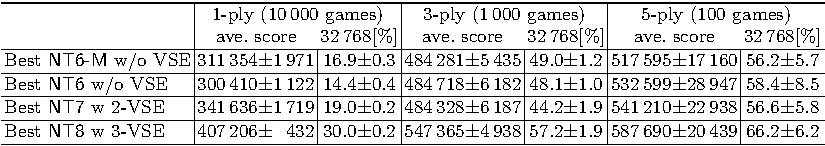
\includegraphics[width=.99\linewidth]{figures/table-exp4.pdf}
\end{table}

Using the best networks, the overall ranking was again \textsf{NT8} $>$ \textsf{NT7} $>$ \textsf{NT6} $\approx$ \textsf{NT6-M}.
For the case combined with 5-ply Expectimax search, the performance gap between \textsf{NT8} and \textsf{NT6-M} was about 70\,000, which was sufficiently larger than the standard deviation.
These results lead us to conclude that combining VSE with larger tuple sizes is highly effective for 2048.

% LocalWords:  Guei et al VSE Ja skowski lookahead overfitting
